\subsection{NUMA-Aware Cache Management}
\label{caching}
Remote caching
Instead of dynamically balancing the NVLink we might start caching remote data 
by putting some of the hardware budget dedicated to the mem-side L2 on a gpu 
side for RC. 
Graph 3: baseline is 1x NVLink with mem-side 4MB L2. Upper bound here is 1x 
NVLink with mem-side 4MB L2 and gpu-side 4MB RC. And then we compare: 4MB L2 + 
128KB RC (tiny RC), 2MB L2 + 2MB RC (half RC), 128KB L2 + 4MB RC (whole RC), 
128KB L2 + 4MB RC but RC can cache both local and remote data. We improve the 
performance on average by XX\%. The main takeaway is that different benchmarks 
prefer different configurations -> motivation for dynamic cache partitioning. 
(Not sure if want to show this? Do we care? Is it important?) What’s the cost of 
invalidation? Especially in case where we allow RC to cache both local and 
remote data, how much we lose by extending the coherency to RC caches. 
(Not sure if want to show this? Do we care? Is it important?) Write-back or 
write-though RC? Some benchmarks prefer WT some WB
Dynamic cache partitioning. Can we try and capture different static 
configurations with one dynamic RC way-partitioning policy? How far we are from 
the upper bound (4MB L2 + 4MB RC)? Is there a difference among GPUs running the 
same benchmark? 
Dynamic NVLink + Dynamic cache partitioning. Combining these two, how far we are 
from the ultimate upper bound which is 2x NVLink + 4MB L2 + 4MB RC. How far we 
are from the 4x larger single-GPU when it comes to scalability?

\begin{figure*}[t]
    \centering
    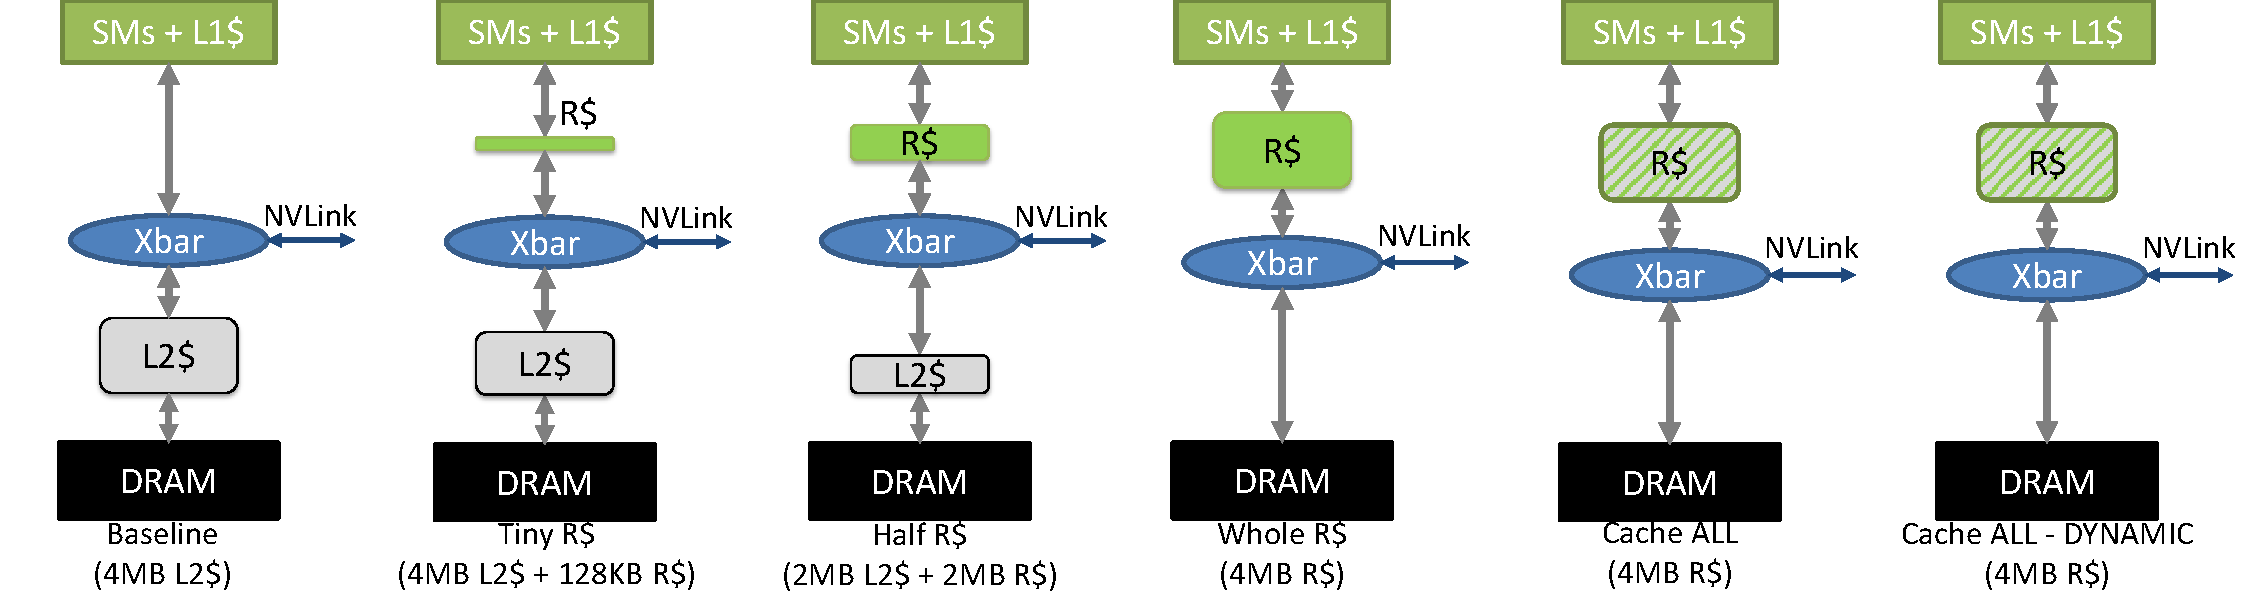
\includegraphics[width=1.0\textwidth]{figures/cache_configurations.pdf}
    \caption{Potential L2 cache organizations to balance capacity between NUMA remote
    local NUMA memory systems.}
    \label{fig:cacheorg}
\end{figure*}

\begin{figure*}[tp]
    \centering
    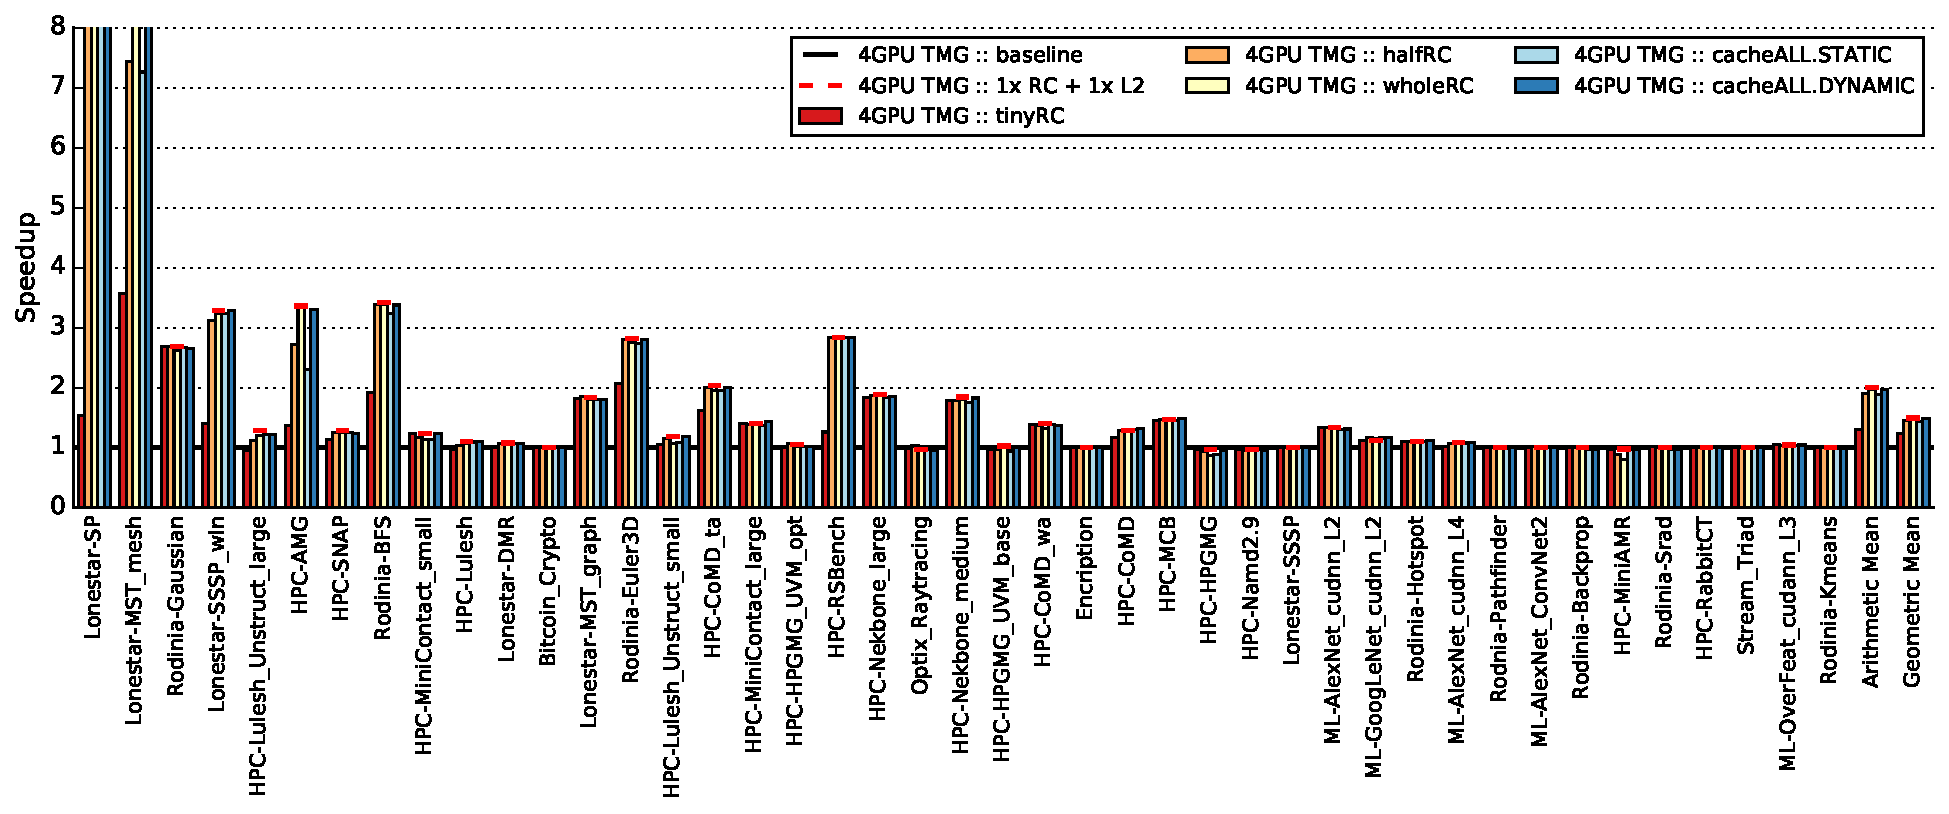
\includegraphics[width=1.0\textwidth]{figures/plot_remote_cache_WB.pdf}
    \caption{Performance comparison of static and dynamic L2 cache organizations
    in a 4-socket NUMA-GPU system.}
    \label{fig:caching}
\end{figure*}

\subsubsection{Results}
Results here

\begin{figure}[t]
    \centering
    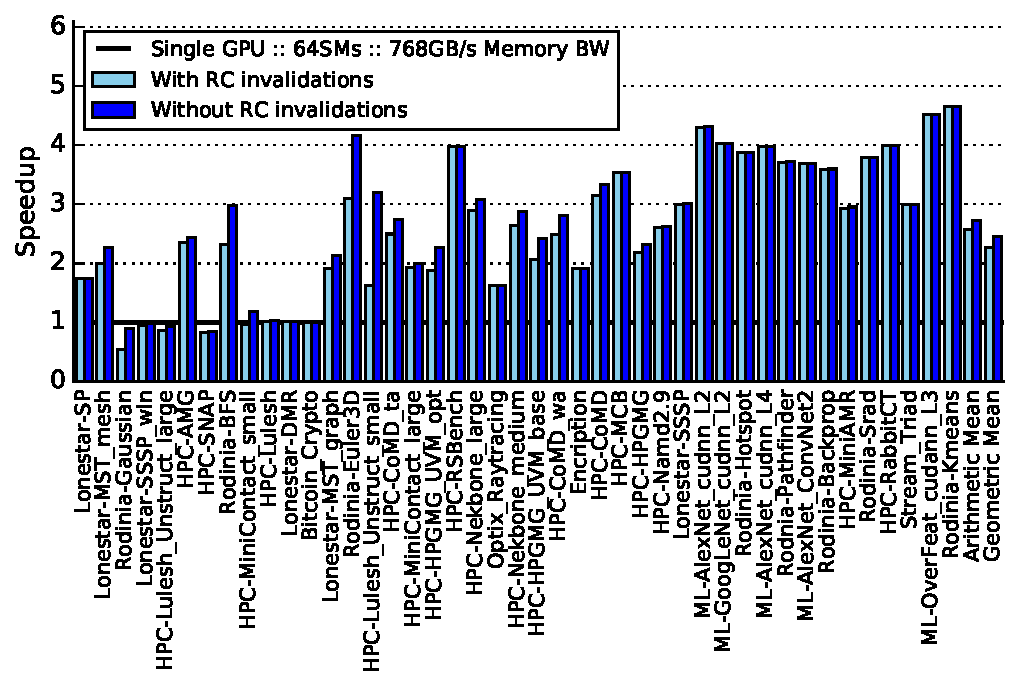
\includegraphics[width=1.0\columnwidth]{figures/plot_no_inval_WB.pdf}
    \caption{Performance overhead of extending current GPU software based coherence
    into the GPU L2 caches.}
    \label{fig:invalidations}
\end{figure}